\documentclass{standalone}

% ==== Essential Packages ====
\usepackage{tikz}
\usepackage{xcolor}
\definecolor{berkeleyblue}{RGB}{0, 50, 98}
\definecolor{berkeleygold}{RGB}{253, 181, 21}

% ==== Custom Colors ====
\definecolor{softyellow}{HTML}{F2D648}

\begin{document}

\begin{center}
    \begin{columns}[T]
  \column{0.6\textwidth}
  \textcolor{berkeleyblue}{\textbf{Experimental Next Steps}}
  
  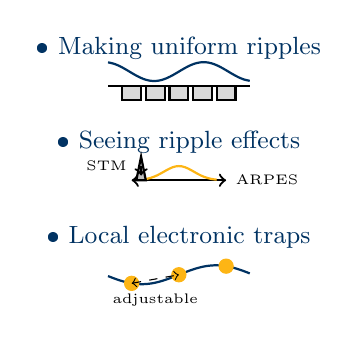
\begin{tikzpicture}[scale=0.6]
    % Substrate engineering - simplified text
    \node[font=\small, berkeleyblue] at (0,0) {• Making uniform ripples};
    \begin{scope}[shift={(0,-0.8)}]
      \draw[thick] (-1.5,0) -- (1.5,0);
      \foreach \x in {-1,-0.5,0,0.5,1} {
        \draw[thick, fill=gray!30] (\x-0.2,-0.3) rectangle (\x+0.2,0);
      }
      \draw[thick, berkeleyblue] plot[smooth, domain=-1.5:1.5] 
        (\x, {0.3+0.2*sin(3*\x*180/pi)});
    \end{scope}
    
    % STM/ARPES characterization - simplified text
    \node[font=\small, berkeleyblue] at (0,-2) {• Seeing ripple effects};
    \begin{scope}[shift={(0,-2.8)}]
      \draw[thick, <->] (-1,0) -- (1,0);
      \draw[thick, berkeleygold] plot[smooth, domain=-0.8:0.8] 
        (\x, {0.3*exp(-5*\x*\x)});
      \node[right, font=\tiny] at (1,0) {ARPES};
      
      % STM tip
      \draw[thick, fill=gray!50] (-0.8,0.5) -- (-0.9,0) -- (-0.7,0) -- cycle;
      \draw[thick, ->] (-0.8,0.3) -- (-0.8,0.1);
      \node[left, font=\tiny] at (-0.9,0.3) {STM};
    \end{scope}
    
    % Tunable quantum dots - simplified text
    \node[font=\small, berkeleyblue] at (0,-4) {• Local electronic traps};
    \begin{scope}[shift={(0,-4.8)}]
      \draw[thick, berkeleyblue] plot[smooth, domain=-1.5:1.5] 
        (\x, {0.2*sin(2*\x*180/pi)});
      \foreach \x in {-1,0,1} {
        \filldraw[berkeleygold] (\x,{0.2*sin(2*\x*180/pi)}) circle (0.15);
      }
      \draw[<->, dashed] (-1,{0.2*sin(2*(-1)*180/pi)}) -- (0,{0.2*sin(2*0*180/pi)});
      \node[font=\tiny, below] at (-0.5,-0.2) {adjustable};
    \end{scope}
  \end{tikzpicture}
  
  \column{0.4\textwidth}
  \textcolor{berkeleyblue}{\textbf{Theory Directions}}
  
  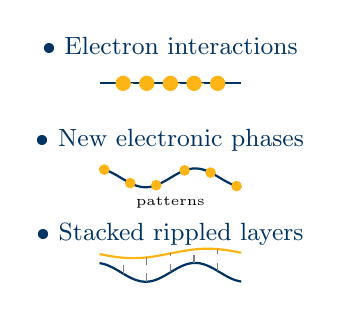
\begin{tikzpicture}[scale=0.6]
    % Many-body interactions - simplified text
    \node[font=\small, berkeleyblue] at (0,0) {• Electron interactions};
    \begin{scope}[shift={(0,-0.8)}]
      \draw[thick, berkeleyblue] (-1.5,0) -- (1.5,0);
      \foreach \x in {-1,-0.5,0,0.5,1} {
        \filldraw[berkeleygold] (\x,0) circle (0.15);
      }
      \draw[<->, dashed, berkeleygold] (-1,0) -- (-0.5,0);
      \draw[<->, dashed, berkeleygold] (0,0) -- (0.5,0);
      \draw[<->, dashed, berkeleygold] (0.5,0) -- (1,0);
    \end{scope}
    
    % Ripple-induced states - simplified text
    \node[font=\small, berkeleyblue] at (0,-2) {• New electronic phases};
    \begin{scope}[shift={(0,-2.8)}]
      \draw[thick, berkeleyblue] plot[smooth, domain=-1.5:1.5] 
        (\x, {0.2*sin(3*\x*180/pi)});
      \foreach \x in {-1.4,-0.85,-0.3,0.3,0.85,1.4} {
        \filldraw[berkeleygold] (\x,{0.2*sin(3*\x*180/pi)}) circle (0.1);
      }
      \node[font=\tiny, below] at (0,-0.2) {patterns};
    \end{scope}
    
    % Emergent properties - simplified text
    \node[font=\small, berkeleyblue] at (0,-4) {• Stacked rippled layers};
    \begin{scope}[shift={(0,-4.8)}]
      % Layer 1
      \draw[thick, berkeleyblue] plot[smooth, domain=-1.5:1.5] 
        (\x, {0.2*sin(3*\x*180/pi)});
      % Layer 2
      \draw[thick, berkeleygold] plot[smooth, domain=-1.5:1.5] 
        (\x, {0.4+0.1*sin(2*\x*180/pi)});
      % Coupling
      \foreach \x in {-1,-0.5,0,0.5,1} {
        \draw[dashed, gray] (\x,{0.2*sin(3*\x*180/pi)}) -- (\x,{0.4+0.1*sin(2*\x*180/pi)});
      }
    \end{scope}
  \end{tikzpicture}
\end{columns}
\end{center}

\end{document}
